\subsection{Central Limit Theorem}


Under certain conditions, the normal distribution can be used to approximate probabilities for linear combinations of random variables having a non-normal distribution. This follows from the Central Limit Theorem (C.L.T.). 

The normal distribution is commonly used because it tends to approximate the distribution of sums of random variables.


\begin{theorem}[\textbf{Central Limit Theorem}]
    \phantom{}  \\
    If $X_1, X_2, \ldots, X_n$ are \textbf{independent} random variables all having the \textbf{same distribution},
    with mean $\mu$ and variance $\sigma^2$, then as $n \to \infty$, the cumulative distribution
    function (c.d.f.) of the random variable
    \[{\color{blue} Z \approx} \frac{\dis \sum_{i=1}^n X_i - n\mu}{\sigma \sqrt{n}} = \frac{S_n - n\mu}{\sigma \sqrt{n}}\]
    approaches the $N(0, 1)$ cumulative distribution function. Similarly, the cumulative distribution
    function of 
    \[{\color{blue} Z \approx} \frac{\overline{X} - \mu}{\frac{\sigma}{\sqrt{n}}}\]
    approaches the $N(0, 1)$ cumulative distribution function.
\end{theorem}

\begin{remark}
    For large $n$, we have
    \begin{itemize}
        \item $S_n = \displaystyle \sum_{i=1}^{n} X_i \sim \text{N}(n\mu, n\sigma^2)$.
        \item $\overline{X} = \frac{1}{n} \displaystyle \sum_{i=1}^{n} X_i \sim \text{N}(\mu, \frac{\sigma^2}{n})$.
    \end{itemize}
    If $X_i$'s themselves have normal distributions, then $S_n$ and $\overline{X}$ have \textbf{exactly} normal distributions $\forall n$. Otherwise, $S_n$ and $\overline{X}$ have \textbf{approximately} normal distributions.
\end{remark}

\pagebreak

\begin{note}
    \phantom{}
    \begin{itemize}
        \item Although this theorem is about limits, we will use it when $n$ is large, but finite.
        \item This theorem works for all distributions except those whose $\mu$ and $\sigma^2$ do not exist.
        \item The accuracy of the approximation depends on $n$ (bigger is better) and on the actual distribution $X_i$'s. It works well for small $n$ when $X_i$'s p.d.f. is close to symmetric.
    \end{itemize}
\end{note}

\begin{theorem}[\textbf{The Law of Large Numbers}]
    \phantom{}\\
    Draw simple random samples of size $n$ at random from a large population with mean $\mu$. As the number of observations drawn increases (i.e. as $n \to \infty$), then the sample mean $\overline{X}$ approaches the population mean $\mu$.
\end{theorem}

General idea of the C.L.T. is that it takes any distribution and makes it normal.
\begin{figure}[htbp]
    \center
    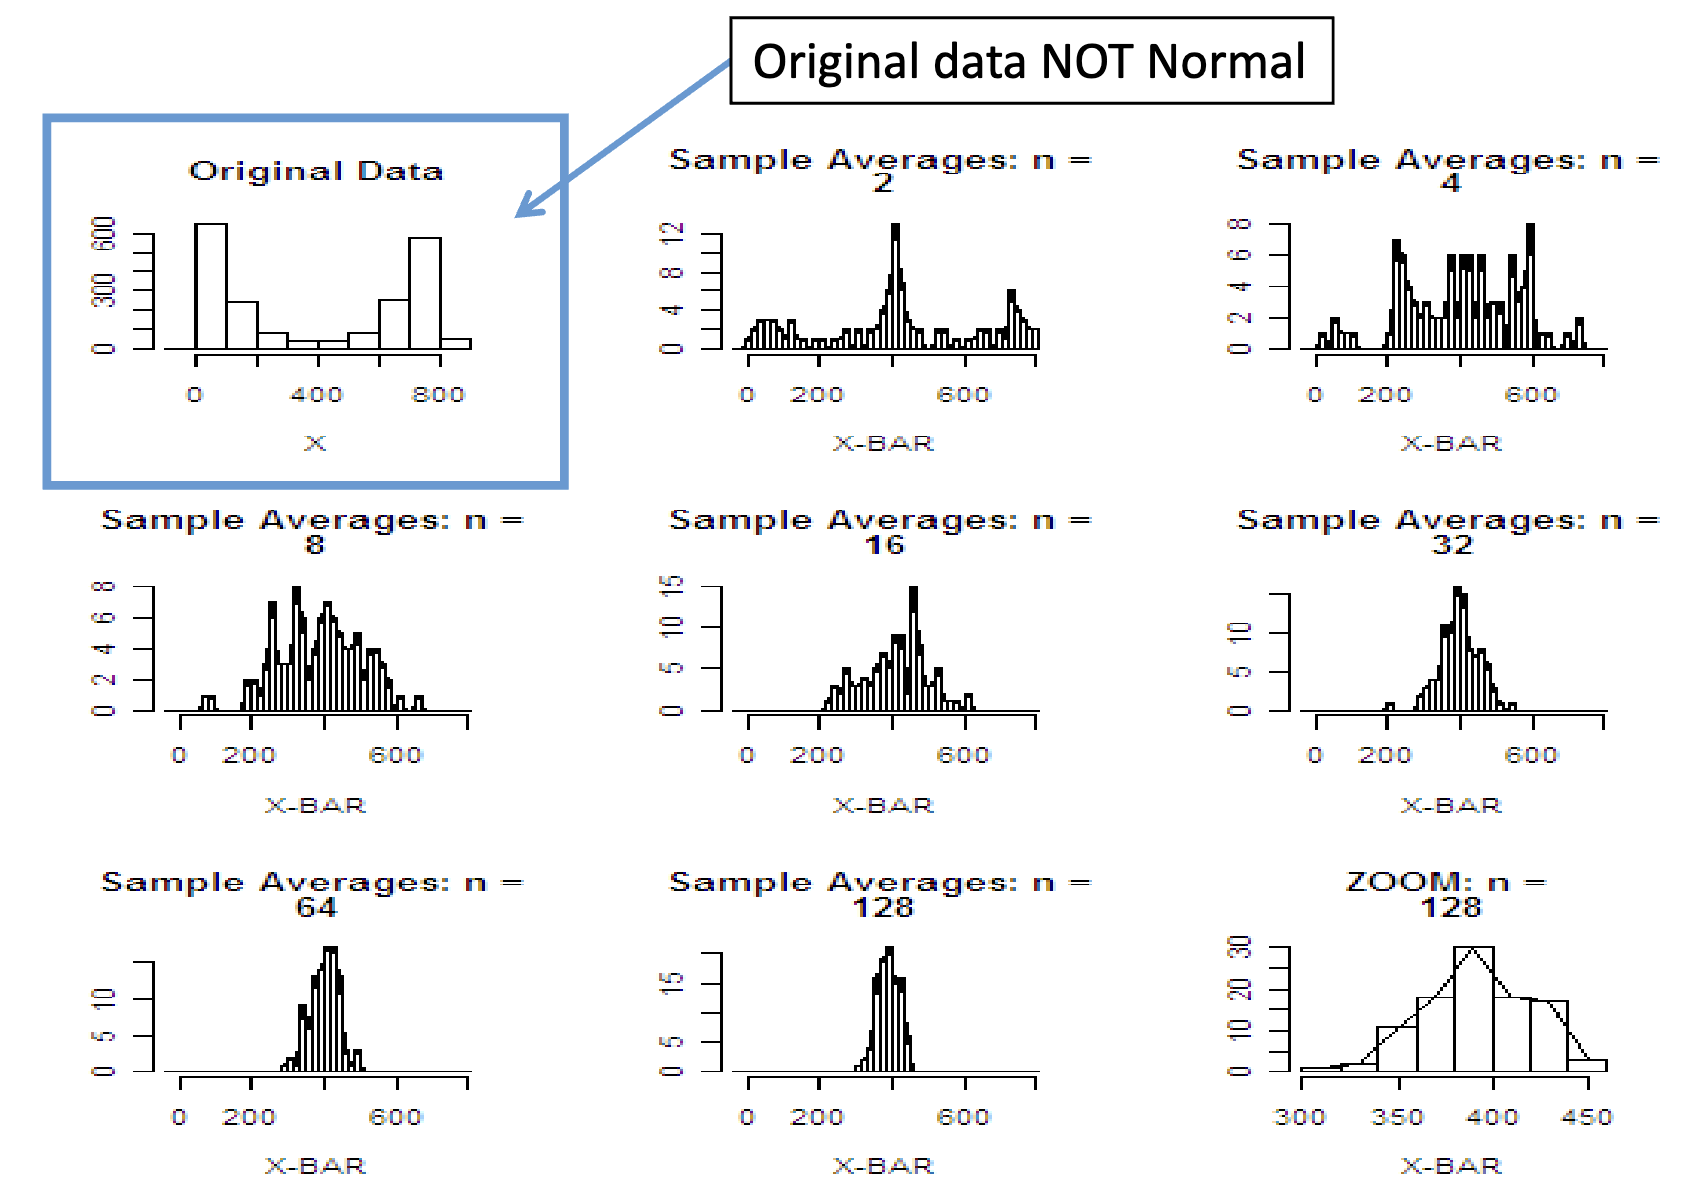
\includegraphics[scale=0.4]{img/CLT-ex.png}
    \caption{Visualizing the idea of CLT.}
\end{figure}

\begin{note}
    The distribution of sample means becomes normal as the sample size increases. Also, the sample mean converges to the population mean when $n$ becomes larger.
\end{note}


\pagebreak


\begin{example}
    Suppose fires reported to a fire station satisfy the conditions for a Poisson process, with a mean of 1 fire every 4 hours. Find the probability the $500^{\text{th}}$ fire of the year is reported on the $84^{\text{th}}$ day of the year.

    \textbf{Solution:} Let $X_i =$ time beteen $(i-1)^{\text{st}}$ and the $i^{\text{th}}$ fires ($X_1 =$ time to the first fire). Then, these $X_i$'s are independent and identically distributed as: $X_i \sim \text{Exp}(\theta = 4 \text{ hrs} = \frac{1}{6} \text{ day})$, since $\lambda = \frac{1}{4}$ fires per hour.

    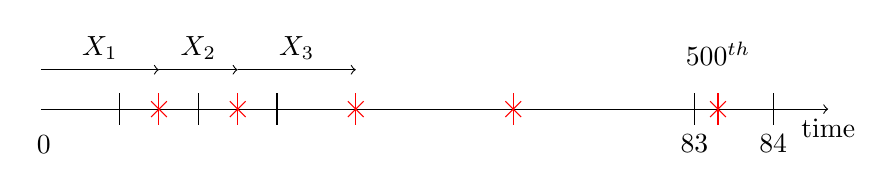
\begin{tikzpicture}
        % Draw the horizontal axis
        \draw[->] (0,0) -- (10,0) node[anchor=north] {time};
        
        % Draw the vertical lines and labels
        \foreach \x in {1, 2, 3} {
            \draw (\x,0.2) -- (\x,-0.2);
        }
        
        % Draw the crosses and labels for 83 and 84
        \foreach \x in {1.5, 2.5, 4, 6, 8.6} {
            \draw[red] (\x,0.2) -- (\x,-0.2);
            \draw[red] (\x-0.1,0.1) -- (\x+0.1,-0.1);
            \draw[red] (\x-0.1,-0.1) -- (\x+0.1,0.1);
        }
        
        \draw (8.3,0.2) -- (8.3,-0.2) node[anchor=north] {83};
        \draw (9.3,0.2) -- (9.3,-0.2) node[anchor=north] {84};
        
        % Draw the arrows for X1, X2, X3
        \draw[->] (0,0.5) -- (1.5,0.5) node[midway,above] {$X_1$};
        \draw[->] (1.5,0.5) -- (2.5,0.5) node[midway,above] {$X_2$};
        \draw[->] (2.5,0.5) -- (4,0.5) node[midway,above] {$X_3$};
        \node at (8.6,0.7) {$500^{\text{th}}$};
        
        % Add the 0 and 1 labels on the left
        \node[anchor=east] at (0.25,-0.45) {0};
        % \node[anchor=east] at (0.78,-0.45) {1};
    \end{tikzpicture}

    We want to find $P \left( 83 < \underbrace{\displaystyle \sum_{i=1}^{500} X_i}_{S_{500}} \leq 84 \right)$. By the Central Limit Theorem, $S_{500} = \displaystyle \sum_{i=1}^{500} X_i$ has approximately \vspace{-2mm}

    a $\text{N}(500\mu , 500\sigma^2) = \text{N}(\frac{500}{6}, \frac{500}{36})$ distribution. 
    \begin{align*}
        P(83 < S_{500} \leq 84) &\approx P \left( \frac{83 - \frac{500}{6}}{\sqrt{\frac{500}{36}}} < Z \leq \frac{84 - \frac{500}{6}}{\sqrt{\frac{500}{36}}} \right) \\
        &= P(-0.09 < Z \leq 0.19) \\
        &\vdots \\
        &= 0.57142 + 0.53586 - 1 \\
        &= 0.10728.
    \end{align*}
\end{example}

\begin{note}
    In this example, we used the normal distribution to approximate a continuous random variable (i.e. the exponential distribution). When approximating discrete random variables, we have to make a small adjustment, see next page!
\end{note}


\pagebreak


\begin{remark}[\textbf{Continuity Correction}]
    \phantom{}\\
    When approximating a discrete random variable, a slight adjustment is required to improve the approximation. 

For example, we are in a `100-cup challenge' where $P(\text{winning cup}) = \frac{1}{6}$, we bought 100 cups to see how many times we win. We want to find the probability of having between 15 to 20 winning cups. 

Let $X_i = $ whether the $i^{\text{th}}$ cup is a winning cup. Then $X_i \sim \text{Binomial}(n=1,p=\frac{1}{6})$ for $i = 1,2,\ldots,100$. And $\expect{X_i} = \frac{1}{6}$, $\Var{X_i} = \frac{5}{36}$, with $S_{100} = \displaystyle \sum_{i=1}^{100} X_i = $ total number of winning cups. By the CLT, we have $S_{100}$ approximately have $\text{N}(\frac{100}{6}, \frac{500}{36})$, we'll see a theorem below about this. Then,
\[
    P(15 \leq S_{100} \leq 20) = P(-0.447 \leq Z \leq 0.894) = 0.487.
\]
If we compute the exact probability using $S_{100} \sim \text{Binomial}(100, \frac{1}{6})$, we get $P(15 \leq S_{100} \leq 20) = 0.561$. This is quite off!

Since $X_i$ are discrete, so $S_{100}$ is also discrete and cannot take non-integer values. In this case, the approximation is underestimate as seen in Figure 14 (part of $X=15$ and $X = 20$ are not included by the normal approximation in {\color{blue} blue}), so subtract 0.5 to get $P(14.5 \leq S_{100} \leq 20.5)$, which gives a better approximation.

\begin{figure}[!htb]
    \begin{minipage}{0.5\textwidth}
      \centering
      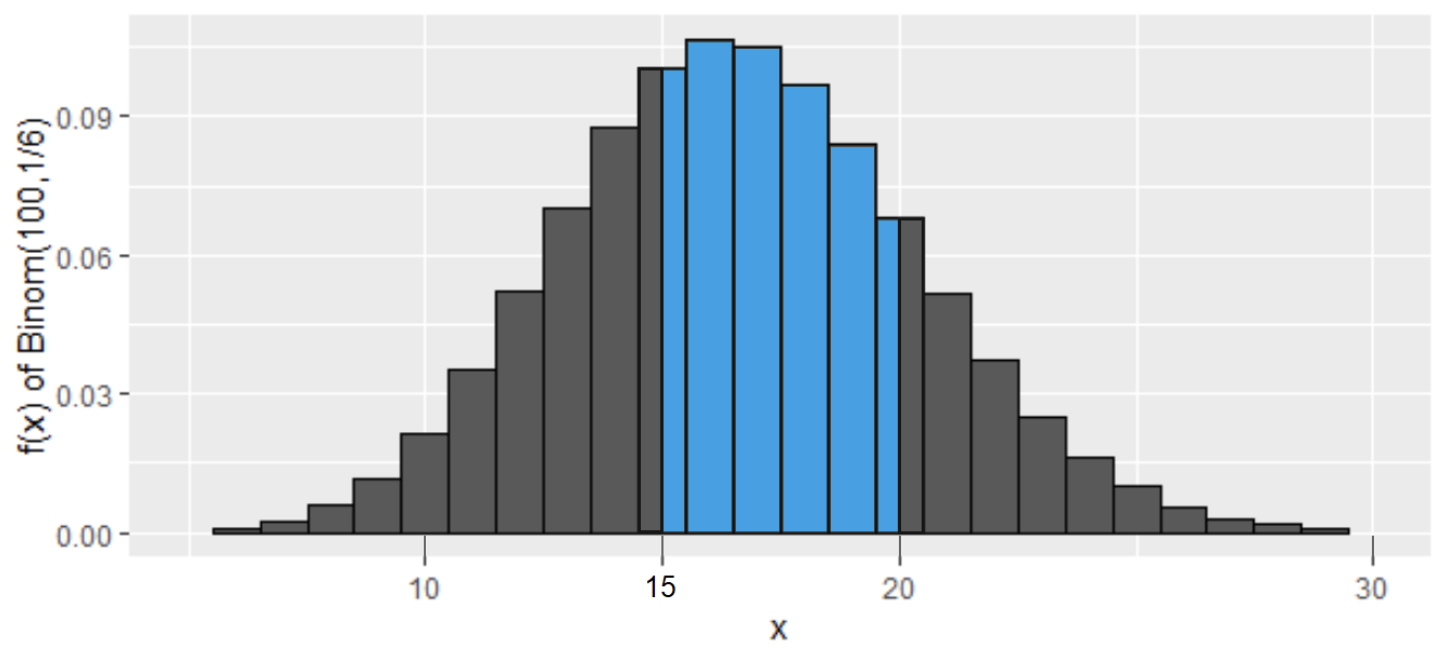
\includegraphics[width=1\linewidth]{img/without-adjustment.png}
      \caption{Without adjustment (underestimate).}
    \end{minipage}\hfill
    \begin{minipage}{0.5\textwidth}
      \centering
      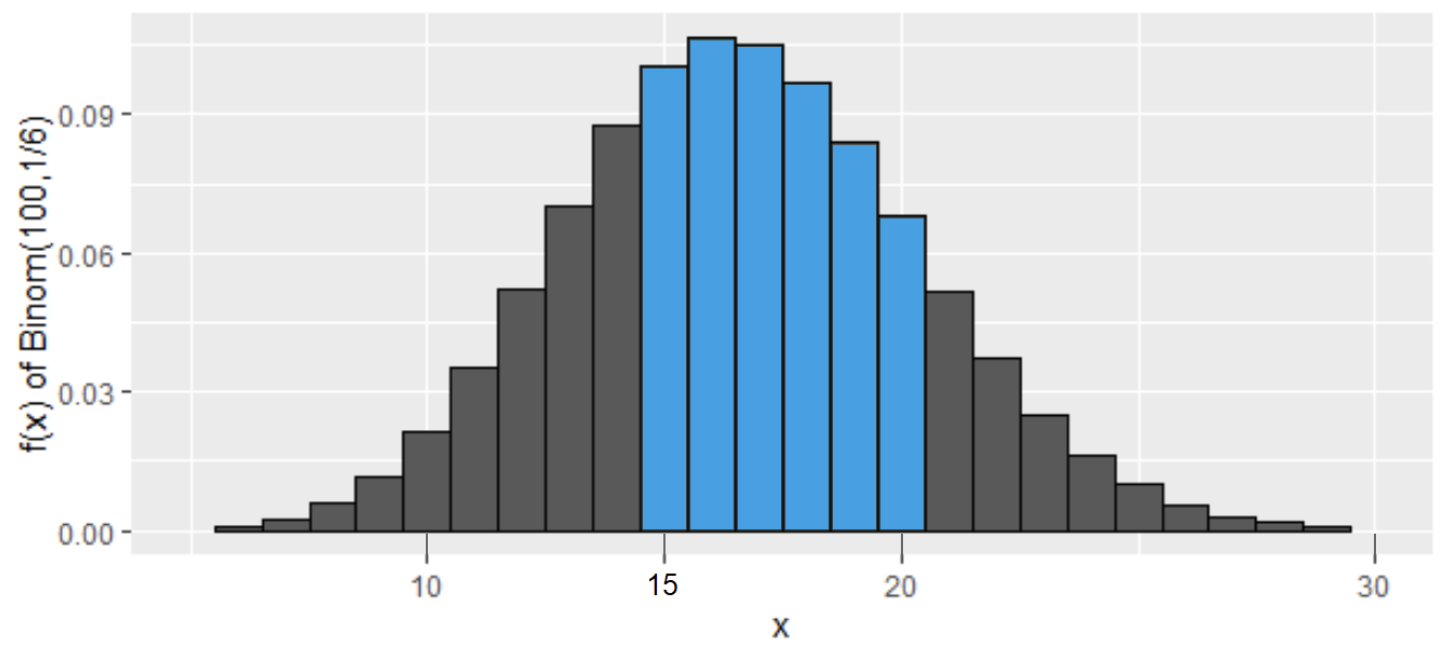
\includegraphics[width=1\linewidth]{img/with-adjustment.png}
      \caption{With adjustment (better).}
    \end{minipage}
 \end{figure}

 $P(14.5 \leq S_{100} \leq 20.5) = 0.568$, which is way better!

 This adjustment is called the ``\textbf{Continuity Correction}''.
\end{remark}

\begin{note}
    \phantom{}
    \begin{itemize}
        \item It is only applied when using a \textbf{continous} distribution to approximate a \textbf{discrete} one.
        \item Quick sketch to see whether to add or subtracct 0.5 (see below proposition).
    \end{itemize}
\end{note}

\begin{proposition}[\textbf{Continuity Correction Rules}]
    \phantom{}\
    \begin{itemize}
        \item $P(X > n)$, use $P(X > n + 0.5)$.
        \item $P(X \geq n)$, use $P(X > n - 0.5)$.
        \item $P(X > n)$, use $P(X < n - 0.5)$.
        \item $P(X \leq n)$, use $P(X < n + 0.5)$.
        \item $P(a < X < b)$, use $P(a + 0.5 \leq X \leq b - 0.5)$.
        \item $P(a \leq X \leq b)$, use $P(a - 0.5 \leq X \leq b + 0.5)$.
        \item $P(X = n)$, use $P(n-0.5 \leq X \leq n + 0.5)$.
    \end{itemize}
\end{proposition}

\begin{theorem}[\textbf{Normal Approximation to Poisson}]
    \phantom{}  \\
    Suppose $X \sim Poisson(\mu)$. Then the cumulative distribution function of the standarized
    random variable \vspace{-2mm}
    \[Z = \frac{X - \mu}{\sqrt{\mu}}\]
    approaches that of a standard Normal random variable as $\mu \to \infty$.
\end{theorem}

\begin{remark}
    We have $X \sim \text{N}(\mu,\mu)$, where $\mu = \lambda t$. Approximation will be good when $\mu > 5$.
\end{remark}

\begin{theorem}[\textbf{Normal Approximation to Binomial}]
    \phantom{}  \\
    Suppose $X \sim Binomial(n, p)$. Then for large $n$, the random variable \vspace{-1mm}
    \[W = \frac{X - np}{\sqrt{np(1 - p)}}\]
    has approximately a $N(0, 1)$ distribution.
\end{theorem}

\begin{remark}
    We write $\frac{X - np}{\sqrt{np(1 - p)}} \sim \text{N}(0,1)$ or $X \sim \text{N}(np,np(1-p))$. \vspace{-1mm} \\
\end{remark}


\begin{example}
    Suppose $X \sim \text{Poisson}(9)$. Use the Normal approximation to approximate $P(X > 9)$, and compare with the true value.

    By Normal approximation to Poisson, we have $Z = \frac{X-\mu}{\sqrt{\mu}}$. Using continuity correction, \vspace{-3mm}
    \[
        P(X > 9) \approx P(X > 9 \text{ } {\color{blue} + \text{ } 0.5}) = P \left( Z > \frac{9.5 - 9}{\sqrt{9}} \right) = P(Z > 0.17) = 0.4324.
    \]
    Note: the true value is 0.4126.
\end{example}

\begin{example}
    Suppose $X \sim \text{Binomial}(20,0.4)$. Find the approximate probability $P(4 \leq X \leq 12)$ and compare it to the true value.

    \textbf{Solution:} Note that $\expect{X} = np = 8$ and $\Var{X} = np(1-p) = 4.8$. By the Normal approximation to the Binomial, we have $X \sim \text{N}(8,4.8)$ approximately.
    \begin{align*}
        P(4 \leq X \leq 12) &\approx P(4 \text{ } {\color{blue} - \text{ } 0.5} \leq X \leq 12 \text{ } {\color{blue} + \text{ } 0.5}) \\
        &= P \left( \frac{3.5 - 8}{\sqrt{4.8}} \leq \frac{X - 8}{\sqrt{4.8}} \leq \frac{12.5 - 8}{\sqrt{4.8}} \right) \\
        &= P(-2.054 \leq Z \leq 2.054) \\
        &\vdots \\
        &= 0.96.
    \end{align*}
    Note: the true value is $\displaystyle \sum_{x=4}^{12} \binom{20}{x} (0.4)^x (0.6)^{20-x} = 0.963$. \\
\end{example}

\begin{example}
    Let $p$ be the proportion of Canadians who think Canada should adopt the US dollar.
    \begin{enumerate}[label=(\alph*)]
        \item Suppose 400 Canadians are randomly chosen and asked their opinion. Let $X$ be the number who say yes. Find the probability that the proportion, $X/400$, of people who say yes is within 0.02 of $p$, if $p$ is 0.20.
        \quad \textbf{Ans:} $2P(Z < 1.06) - 1 = 0.711$.
        \item Find the number, n, who must be surveyed so there is a $95\%$ chance that $X/n$ lies within 0.02 of $p$, when $p$ is unknown.
        
        \textbf{Ans:} $Z = 1.96 = \frac{0.02}{\sqrt{\frac{p(1-p)}{n}}}$. Set $(p(1-p))^\prime = 0$ to find the max $p = 0.5$. Sub in $p = 0.5$ to get $n = 2401$, and this works for all $p$ since it works for the max $p$.
    \end{enumerate}
\end{example}

\pagebreak

\subsection{Moment Generating Functions}

So far, we have seen two functions which characterize a distribution of a random variable:
\begin{itemize}
    \item p.d.f.
    \item c.d.f.
\end{itemize}
However, there is a third function which also \textbf{uniquely} determines a distribution: the \textbf{moment generating function}.


\begin{definition}[\textbf{Moment Generating Functions for Discrete}]
    \phantom{}\\
    Consider a discrete random variable $X$ with probability function $f(x)$. The moment generating function (m.g.f.) of $X$ is defined as \vspace{-3mm}
    \[
        M(t) = \expect{e^{tX}} = \displaystyle \sum_{\text{all $x$}} e^{tx} f(x).
    \]
    We will assume that the moment generating function is defined and finite for values of $t$ in an interval around 0 (i.e. for some $a > 0$, $\displaystyle \sum_{x} e^{tx} f(x) < \infty \; \forall t \in [-a,a]$).
\end{definition}

The m.g.f. of $X$ can be used to evaluate the moments of the random variable $X$, where the \textbf{moments} of $X$ are defined as the \textbf{expectations} of the functions $X^k$ for $k = 1,2,\ldots$. \vspace{-3mm}
\[
    \expect{X^k} \text{ is the $k^{\text{th}}$ moment of $X$.}
\]

\vspace{-3mm}

\begin{example}
    \phantom{}\
    \begin{itemize}
        \item The mean $\mu = \expect{X}$ is the first moment of $X$.
        \item $\expect{X^2}$ is the second moment of $X$ and so on.
    \end{itemize}
\end{example}

\vspace{2mm}

\begin{theorem}
    \phantom{}\\
    Suppose the random variable $X$ has moment generating function $M(t)$ defined $\forall t \in [-a,a]$ for some $a > 0$. Then \vspace{-3mm}
    \[
        \expect{X^k} = M^{(k)}(0) \quad \text{for $k = 1,2,\ldots$}
    \]
    where $M^{(k)}(0) = \dis \frac{\dd^k}{\dd{t^k}} M(t) \, |_{t=0} \quad \text{for } k = 1, 2, \ldots$
\end{theorem}

\pagebreak

\begin{example}[\textbf{MGF for Binomial}]
    \phantom{}\\
    Suppose $X \sim \text{Binomial}(n,p)$. Then its moment generating function is
    \begin{align*}
        M(t) &= \displaystyle \sum_{x=0}^{n} e^{tx} \binom{n}{x} p^x (1-p)^{n-x} \\
        &= \displaystyle \sum_{x=0}^{n} \binom{n}{x} (p e^t)^x (1-p)^{n-x} \\
        &=(pe^t + 1 - p)^n \quad \text{by the Binomial Theorem $\forall t$.}
    \end{align*}
    Therefore, \vspace{-3mm}
    \begin{align*}
        M^\prime(t) &= npe^t \left(pe^t + 1 - p\right)^{n-1} \\
        M^\dprime(t) &= npe^t \left(pe^t + 1 - p\right)^{n-1} + n(n-1)p^2 e^{2t} \left(pe^t + 1 - p\right)^{n-2}
    \end{align*}
    and so
    \begin{align*}
        \expect{X} &= m^\prime(0) = np \\
        \expect{X^2} &= M^\dprime(0) = np + n(n-1)p^2 \\
        \Var{X} &= \expect{X^2} - \left( \expect{X} \right)^2 = np(1-p).
    \end{align*}
\end{example}

\begin{example}[exercise]
    Find the m.g.f. for a Poisson distrubition $X \sim \text{Poisson}(\mu)$. \\
\end{example}

\begin{theorem}[\textbf{Uniqueness Theorem for MGFs}]
    \phantom{}\\
    Suppose that random variables $X$ and $Y$ have moment generating functions $M_X(t)$ and $M_Y(t)$, respectively. If $M_X(t) = M_Y(t) \; \forall t$, then $X$ and $Y$ have the same distribution.
\end{theorem}

The m.g.f. uniquely identifies a distribution. For example, if $X$ has m.g.f.: $e^{2(e^t -1)}$. Then, you can immediately tell that $X \sim \text{Poisson}(2)$.

MGFs can also be used to determine that a sequence of distributions gets closer and closer to some limiting distribution. To show this, suppose that a sequence of probability functions $f_n(x)$ have corresponding moment generating functions: \vspace{-3mm}
\[
    M_n(t) = \displaystyle \sum_{\text{all $x$}} e^{tx} f_n(x).
\]
And suppose that the probability functions $f_n(x)$ converge to another probability function $f(x)$ pointwise in $x$ as $n \to \infty$. Then since
\vspace{-3mm}
\[
    f_n(x) \to f(x) \text{ as $n \to \infty$ for each $x$},
\]
we have \vspace{-3mm}
\[
    \sum_{\text{all $x$}} e^{tx} f_n(x) \to \sum_{\text{all $x$}} e^{tx} f(x) \text{ as $n \to \infty$ for each $t$}.
\]
In other words, $M_n(t)$ converges to $M(t)$, the moment generating function of the limiting distribution.

\textbf{Note:} The converse also holds. Suppose that $X_n$ has m.g.f. $M_n(t)$ and $M_n(t) \to M(t)$ for each $t$, such that $M(t) < \infty$, then
\vspace{-3mm}
\[
    f_n(x) \to f(x) \text{ as $n \to \infty$ for each $x$}.
\]

\begin{example}
    The Poisson approximation of the Binomial distribution when $n$ is very large and $p$ is close to 0.

    $\mu = np \implies p = \frac{\mu}{n}$. Then, the m.g.f. of such a Binomial random variable:
    \begin{align*}
        M(t) &= (pe^t + 1 - 1)^n \\
        &= \left[ 1 + p(e^t -1) \right]^n \\
        &= \left[ 1 + \frac{\mu}{n} (e^t -1) \right]^n.
    \end{align*}
    Now, take the limit of this expression as $n \to \infty$. Since $\dis \lim_{n \to \infty} \left( 1 + \frac{c}{n} \right)^n \to e^c$, we have
    \[
        \lim_{n \to \infty} \left[ 1 + \frac{\mu}{n} (e^t -1) \right]^n = e^{\mu(e^t -1)},
    \]
    and this is the m.g.f. of a Poisson distribution with parameter $\mu$. This shows a little more formally that the Binomial distribution with small $p$ and large $n$ approaches the Poisson distribution with $\mu = np$  as $n \to \infty$.
\end{example}

\pagebreak

\textbf{Moment Generating Function of a Continuous Random Variable}

\begin{definition}[\textbf{Moment Generating Functions for Continous}]
    \phantom{}\\
    Consider a continuous random variable $X$ with probability density function $f(x)$. Then moment generating function of $X$ is defined as
    \vspace{-3mm}
    \[
        M(t) = \expect{e^{tx}} = \displaystyle \int_{-\infty}^{\infty} e^{tx} f(x) \, dx.
    \]
    We will assume that the m.g.f. is defined and finite for values of $t$ in an interval around 0. That is, for some $a > 0$, $\displaystyle \int_{-\infty}^{\infty} e^{tx} f(x) \, dx < \infty \; \forall t \in [-a,a]$.
\end{definition}

\begin{example}
    Suppose that $X \sim \text{Exponential}(\theta)$. Show that the m.g.f. is given by \vspace{-3mm}
    \[
        M(t) = \frac{1}{1 - \theta t} \quad \text{for $t < \frac{1}{\theta}$}.
    \]
    \textbf{Solution:} Recall that $\Gamma(\alpha) = \displaystyle \int_{0}^{\infty} x^{\alpha -1} e^{-x} \, dx$. By definition, we have \vspace{-3mm}
    \begin{align*}
        M(t) &= \displaystyle \int_{0}^{\infty} e^{tx} \lambda e^{-\lambda x} \, dx \\
        &= \lambda \displaystyle \int_{0}^{\infty} x^{1-1} e^{-x(\lambda - t)} \, dx \quad \text{let $u = x(\lambda - t)$}, dx = \frac{du}{\lambda - t} \\
        &= \dis \frac{\lambda}{\lambda - t} \displaystyle \int_{0}^{\infty} \left( \frac{u}{\lambda - t} \right)^{1-1} e^{-u} \, dx \\
        &= \dis \frac{\lambda}{\lambda - t} \displaystyle \int_{0}^{\infty} u^{1-1} e^{-u} \, dx \\
        &= \dis \frac{\lambda}{\lambda - t} \cdot \Gamma(1) \\
        &= \dis \frac{\lambda}{\lambda - t} \\
        &= \dis \frac{1}{1 - \theta t} \quad \text{since $\theta = \frac{1}{\lambda}$}.
    \end{align*}
    Notice that $\lambda - t > 0$ is necessary for the integral to converge, so we have $t < \lambda = \frac{1}{\theta}$.
\end{example}

\pagebreak

\begin{proposition}[\textbf{Summary of MGFs}]
    \phantom{}\\
    For discrete random variables:
    \begin{itemize} \itemsep 1.5pt
        \item If $X \sim \text{Binomial}(n,p)$, then $M(t) = (pe^t + 1 - p)^n$, $t \in \R$.
        \item If $X \sim \text{Poisson}(\mu)$, then $M(t) = e^{\mu (e^t -1)}$, $t \in \R$.
        \item If $X \sim \text{NB}(k,p)$, then $\dis M(t) = \left( \frac{p}{1- (1-p)e^t} \right)^k$, $t < - \ln(1-p)$.
        \item If $X \sim \text{Geometric}(p)$, then $\dis M(t) = \frac{p}{1- (1-p)e^t}$, $t < - \ln(1-p)$.
    \end{itemize}
    For continuous random variables:
    \begin{itemize} \itemsep 1.5pt
        \item If $X \sim \text{U}(k,p)$, then $\dis M(t) = \frac{e^{bt} - e^{at}}{(b-a)t}$, $t \neq 0$.
        \item If $X \sim \text{Exponential}(\theta)$, then $\dis M(t) = \frac{1}{1- \theta t}$, $t < - \frac{1}{\theta}$.
        \item If $X \sim \text{NB}(k,p)$, then $\dis M(t) = e^{\mu t + \frac{\sigma^2 t^2}{2}}$, $t \in \R$.
    \end{itemize}
\end{proposition}

\phantom{}\\

\subsection{Motivariate Moment Generating Functions}

Did-not-have-time-to-cover material. \\
\phantom{}\\
\phantom{}\\
\phantom{}\\
\phantom{}\\
\phantom{}\\
\phantom{}\\
\phantom{}\\
\phantom{}\\
\phantom{}\\
\phantom{}\\
\phantom{}\\
\phantom{}\\
\phantom{}\\
% \vspace{0.5mm}

\begin{center}
    {\LARGE END OF STAT 230!}
\end{center}



\newpage